\documentclass[]{article}
\usepackage{graphicx}
\usepackage{float}
\usepackage{amsmath}
%\usepackage[]{hyperref}
% Title Page
\title{Lab 1}
\author{
	Alex Taglieri
	\\
	Andrew Kacherski
	}

\begin{document}
\maketitle
\newpage
\
\raggedright


\pagenumbering{arabic}
\section{Introduction and Background}
When a spring is pulled, the force it generates is proportional to its displacement from its resting position. The system is described by the following equation:

\begin{equation}\label{fkx}
f=kx
\end{equation}

A consequence of this equation is that it is possible to predict how much force (\textit{f}) is being applied for a given displacement (\textit{x}) and spring force constant (\textit{k}). 

Furthermore, if the system is vertical and a known mass is placed on the end, it is possible to calculate the spring's force constant \textit{k} by observing the change in the mass's displacement. The equation for determining the magnitude of the force that the mass exerts on the spring (when the system is at rest) is the following:

\begin{equation}\label{fma}
f=ma
\end{equation}

Since we are on Earth, \textit{a} can be assumed to be $9.81m/s^2$. Equation \ref{fma} is needed to determine the value of \textit{f} in Equation \ref{fkx} when the system is vertical and stationary.

A more interesting situation arises when the system is no longer stationary. If the mass starts moving up and down, its position follows the following path:

\begin{equation}\label{shm}
x(t)=Acos(\omega t + \phi)
\end{equation}

where \textit{A} is the amplitude of the oscillation (in meters), \textit{$\omega$} is the angular frequency of the oscillation (in rad/sec), and \textit{$\phi$} is the phase offset of the system (in radians). For the purposes of this lab, \textit{A} and \textit{$\phi$} are not interesting.

The value of \textit{$\omega$} is the important one. It can be found if the values of \textit{k} and \textit{m} from Equation \ref{fkx} are known:

\begin{equation}\label{findTheOmega}
\omega = \sqrt{\frac{k}{m}}
\end{equation}

Characterizing the frequency of oscillation of a vertical spring-mass system on Earth requires knowing the values of \textit{k} and \textit{m}.


When two springs are in parallel, their combined \textit{k} value is given by equation \ref{parallelSpring}, which makes sense because each spring develops the force predicted by Equation \ref{fkx} on its own, and parallel vectors can be added together.

\begin{equation}\label{parallelSpring}
k_{parallel} = k_1 + k_2
\end{equation}

and when they are in series, the resultant \textit{k} value is

\begin{equation}\label{seriesSpring}
k_{series}=\frac{1}{\frac{1}{k_1} + \frac{1}{k_2}}
\end{equation}

\section{Procedure}
\raggedright
The general strategy followed in this lab is to determine the \textit{k} value of the spring using Equation \ref{fkx} for different values of \textit{f}, and then to use that \textit{k} value to predict a value for $\omega$. We'll then test the value of $\omega$ experimentally and compare the two values. The procedure will be repeated for one spring, a second spring, and both springs in series.

In order to calculate the k values of the springs, we connected the top of the spring to an apparatus that measures force, and hung the bottom of the mass over a sensor that can detect the height of the spring. The force-measuring apparatus allowed us to determine the value of \textit{f} in Equation \ref{fkx}, and the height sensor let us find the value of \textit{x}. We varied the value of \textit{f} across a range of values to minimize bias and error: masses of 100, 200, 300, 400, 500, and 600 grams were used to give a force varying from .98N to 5.9N. 

Once we had k values that had been calculated statically (with the masses not moving) for each of the springs, we could set the system in motion and observe the frequencies of oscillation of each configuration of springs (spring 1 independently, spring 2 independently, and then both springs in series). This part of the experiment was carried out with a 400g mass at the end of the spring for each iteration of the experiment.

\section{Results}

We found the spring constant of Spring 1 to be 34.04$\pm$.06207 N/m (Figure \ref{Force vs. Displacement for Spring 1}). The value for Spring 2 was 34.78$\pm$2.006 N/m. When both springs were in series we measured a k value of 17.59$\pm$.07221.


\begin{figure}[H]
	\centering
	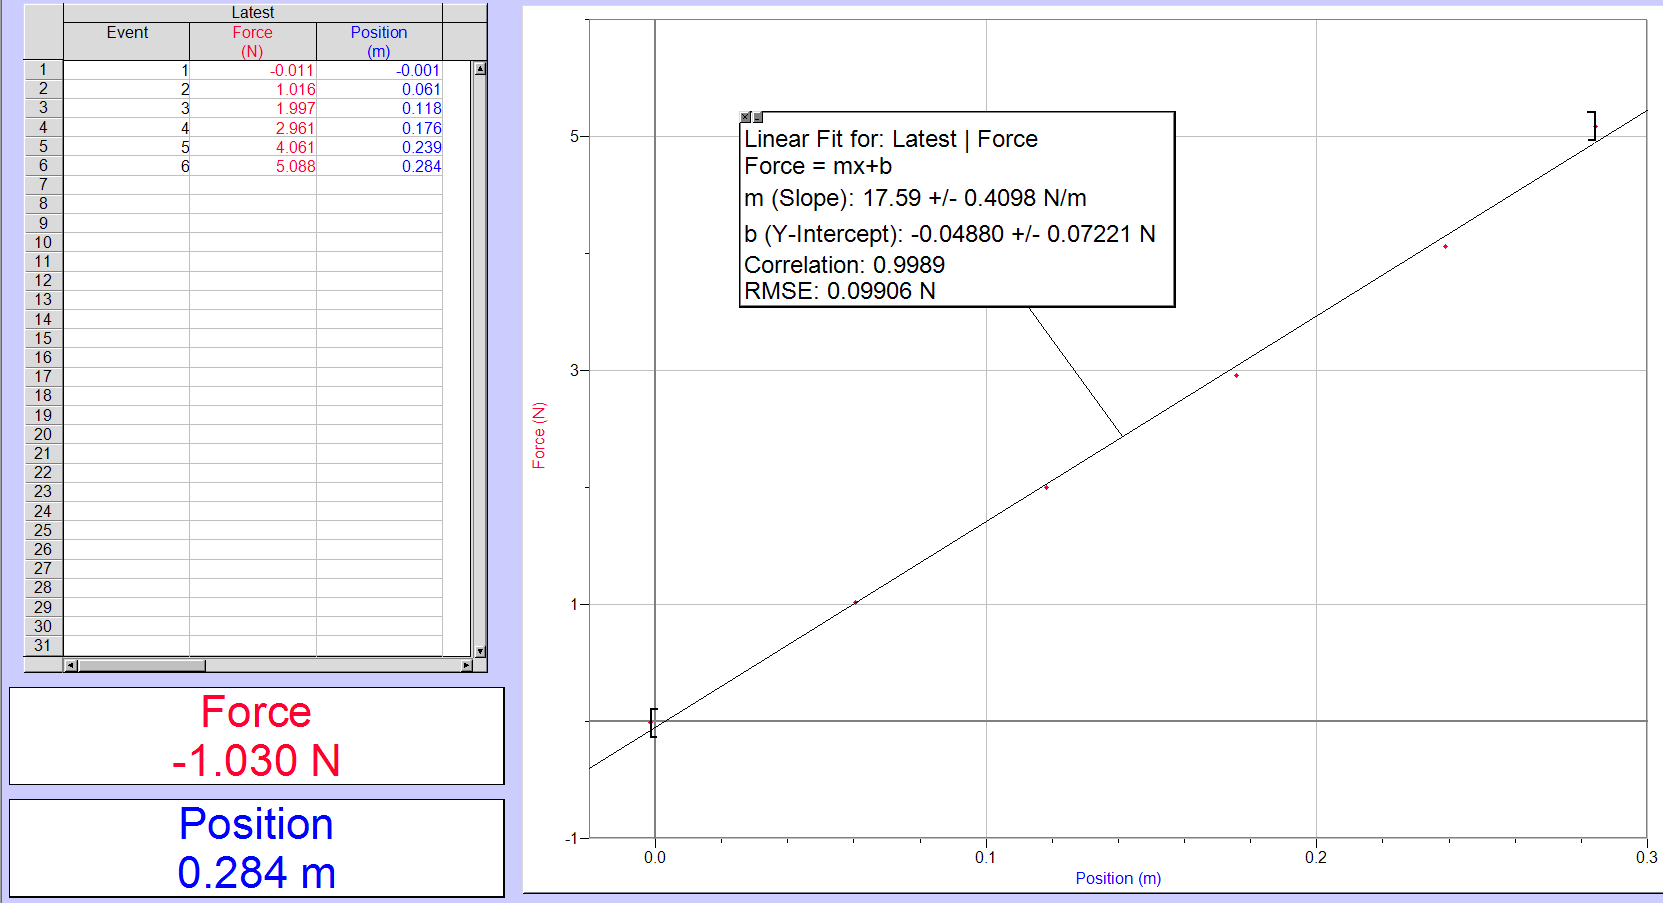
\includegraphics[width=\textwidth]{res/lab_1}
	\caption{Force vs. Displacement for Spring 1}
	\label{Force vs. Displacement for Spring 1}
\end{figure}


When the masses started oscillating, we found that the mass on Spring 1 oscillated at $9.074 \frac{rad}{sec}$ (Figure \ref{fig:Spring 1 Oscillations}), the mass on Spring 2 oscillated at $9.055\frac{rad}{sec}$ (Figure \ref{fig:Spring 2 Oscillations}), and when the mass was hung from both springs in series it oscillated at $5.521\frac{rad}{sec}$ (Figure \ref{fig:Oscillations of Both Springs}).

\begin{figure}[H]
	\centering
	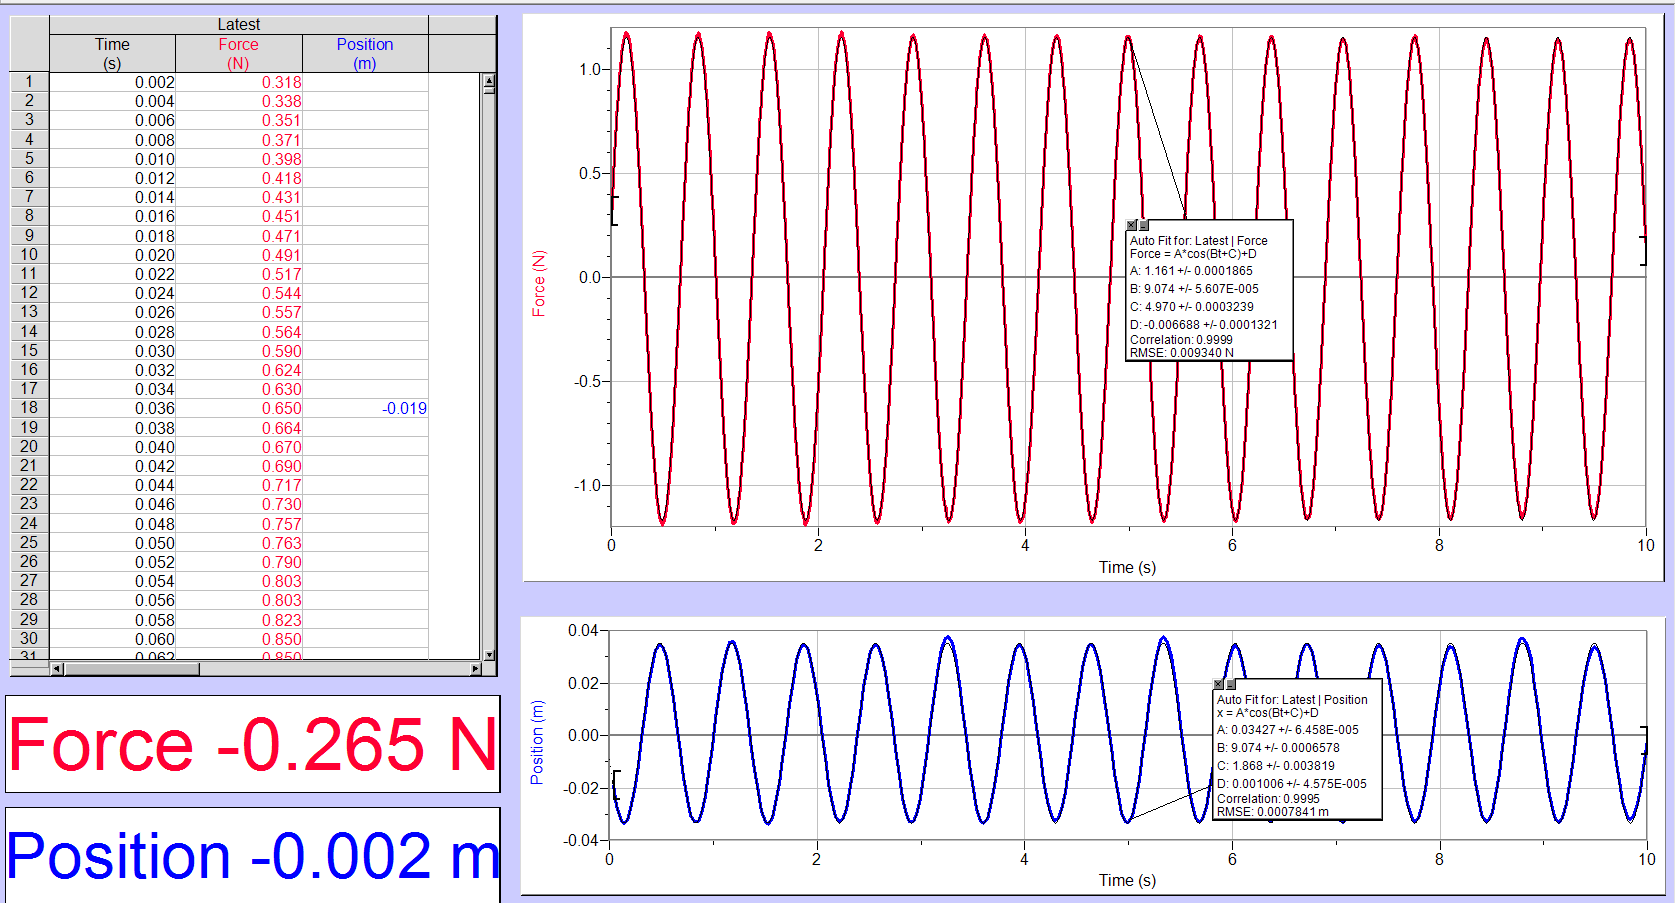
\includegraphics[width=\textwidth]{res/oscillations_spring_1}
	\caption{Spring 1 Oscillations}
	\label{fig:Spring 1 Oscillations}
\end{figure}

\begin{figure}[H]
	\centering
	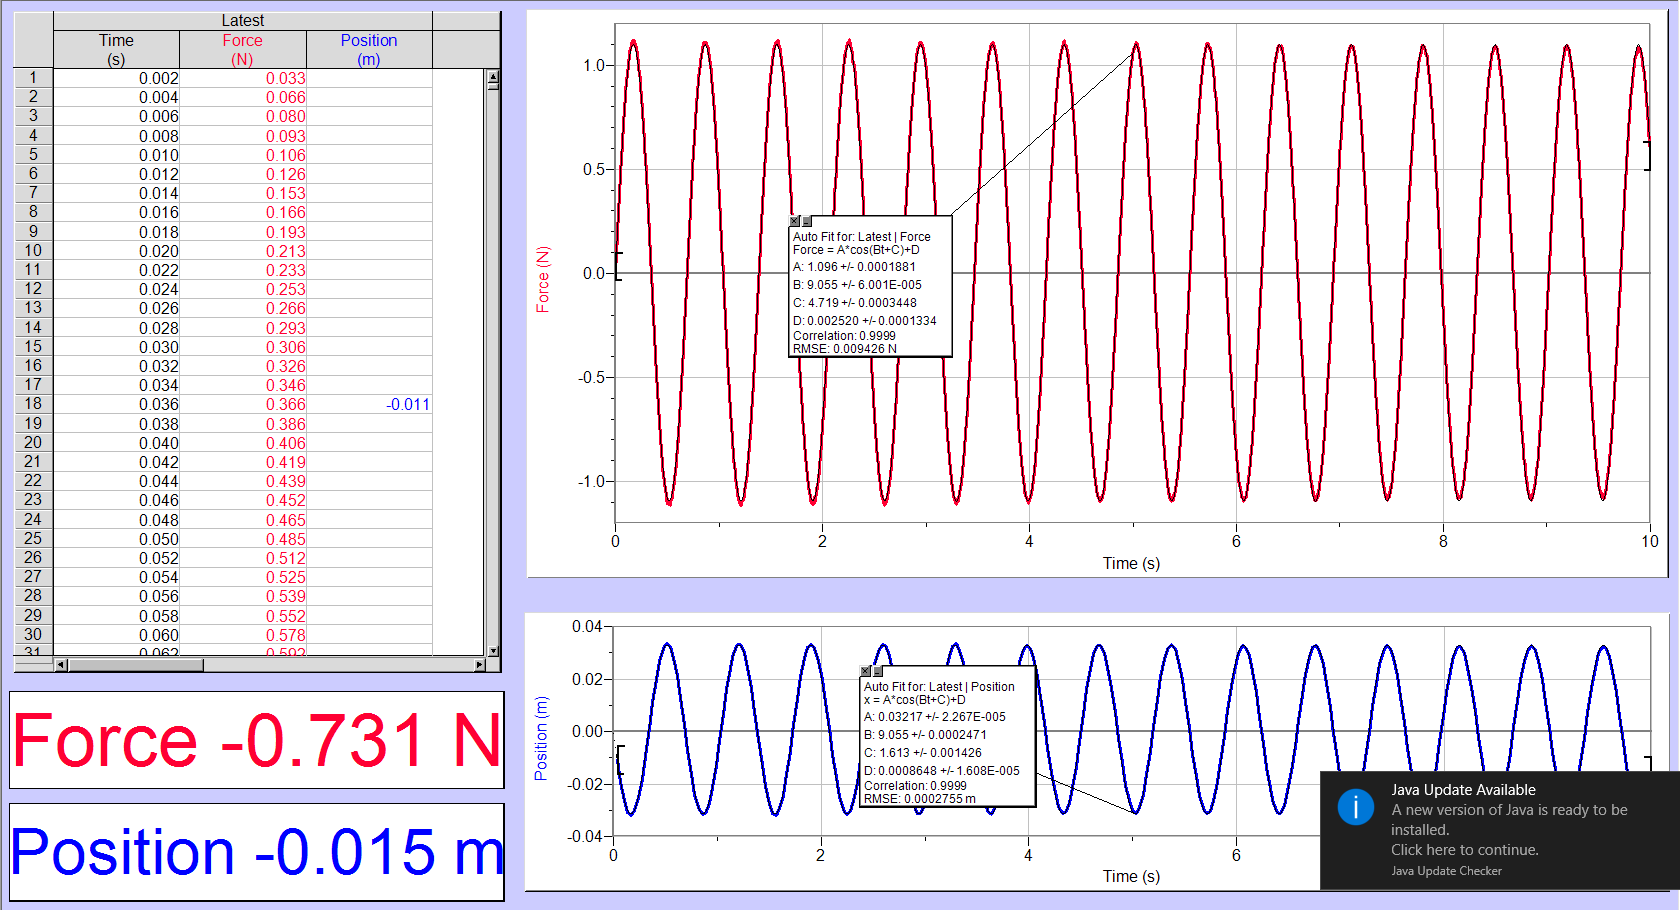
\includegraphics[width=\textwidth]{res/oscillations_spring_2}
	\caption{Spring 2 Oscillations}
	\label{fig:Spring 2 Oscillations}
\end{figure}

\begin{figure}[H]
	\centering
	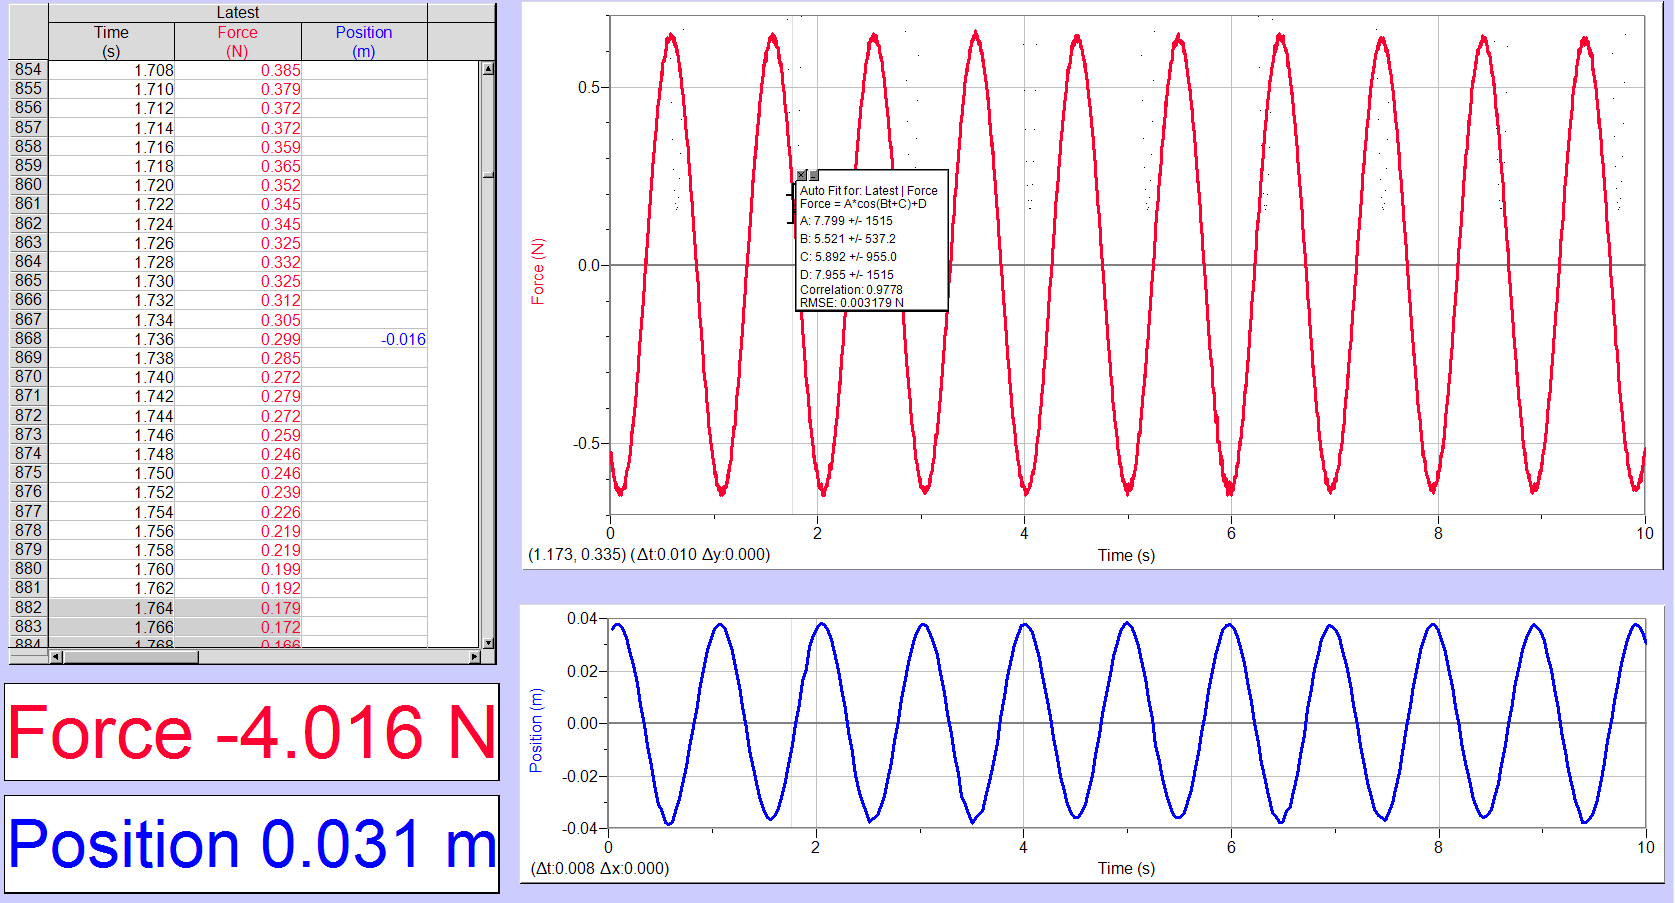
\includegraphics[width=\textwidth]{res/oscillations_both_springs}
	\caption{Oscillations of Both Springs}
	\label{fig:Oscillations of Both Springs}
\end{figure}

\section{Discussion}
The theory predicted that the \textit{k} value of two springs in series would be described by Equation \ref{seriesSpring} (reproduced here for clarity):

\begin{equation*}
k_{series}=\frac{1}{\frac{1}{k_1} + \frac{1}{k_2}} \tag{\ref{seriesSpring}}
\end{equation*}

Plugging numbers in, we find 

\begin{equation}
\frac{1}{\frac{1}{34.04}+\frac{1}{34.78}} = 17.20 N/m
\end{equation}

The measured value was 17.59, which is a 2.2\% error.

Furthermore, Spring 1's \textit{k} value of 34.04 means we should have observed an $\omega $ value of $\sqrt{\frac{34.04}{.4}} = 9.22$. The actual observed value was 9.074, which is 1.6\% away.

Putting the springs in series did, in fact, change their k values according to equation \ref{seriesSpring}.

\end{document}          
